% The MIT License (MIT)
%
% Copyright (c) 2020 Yegor Bugayenko
%
% Permission is hereby granted, free of charge, to any person obtaining a copy
% of this software and associated documentation files (the "Software"), to deal
% in the Software without restriction, including without limitation the rights
% to use, copy, modify, merge, publish, distribute, sublicense, and/or sell
% copies of the Software, and to permit persons to whom the Software is
% furnished to do so, subject to the following conditions:
%
% The above copyright notice and this permission notice shall be included
% in all copies or substantial portions of the Software.
%
% THE SOFTWARE IS PROVIDED "AS IS", WITHOUT WARRANTY OF ANY KIND, EXPRESS OR
% IMPLIED, INCLUDING BUT NOT LIMITED TO THE WARRANTIES OF MERCHANTABILITY,
% FITNESS FOR A PARTICULAR PURPOSE AND NON-INFRINGEMENT. IN NO EVENT SHALL THE
% AUTHORS OR COPYRIGHT HOLDERS BE LIABLE FOR ANY CLAIM, DAMAGES OR OTHER
% LIABILITY, WHETHER IN AN ACTION OF CONTRACT, TORT OR OTHERWISE, ARISING FROM,
% OUT OF OR IN CONNECTION WITH THE SOFTWARE OR THE USE OR OTHER DEALINGS IN THE
% SOFTWARE.

% \documentclass[a4paper,UKenglish,cleveref, autoref]{lipics-v2019}
\documentclass[12pt]{article}
\title{Source Code Volatility Metric}
\author{Yegor Bugayenko}{}{}
% \authorrunning{Yegor Bugayenko}
% \ccsdesc[100]{Software and its engineering~Object oriented languages}
% \keywords{Object-Oriented Programming, Immutability, NCSS}
\usepackage[utf8]{inputenc}
\usepackage[numbers]{natbib}
\bibliographystyle{plainnat}
\usepackage{textcomp}
\usepackage[inline]{enumitem}
\usepackage{amsmath}
\usepackage{graphicx}
\usepackage{pgfplots}
\usepackage{verbatimbox}
\usepackage{interval}
\usepackage{hyperref}
\usepackage{minted}
  \setminted{fontsize=\footnotesize}
  \setminted{breaklines}
  \usemintedstyle{bw}
\newcommand{\code}[1]{\texttt{#1}}
\newenvironment{nicetable}
  {\setlength{\parindent}{0em}\medskip\small}
  {\medskip}
\def\thetotaljavafiles{10023}
\def\thetotalrepos{240}

\begin{document}
\raggedbottom
\maketitle

\begin{abstract}
A new metric was introduced to calculate the distance
between actively modified files in a source code repository
and the files, which are rarely modified and may be considered
as ``dead'' or ``abandoned.'' It was empirically demonstrated that larger repositories
have larger values of the introduced metric.
\end{abstract}

\section{Introduction}

Most software development projects keep their source code in Git~\citet{loeliger2012},
which is the de-facto standard in the industry at the moment, or similar
version control systems. Every system, including open
source products like Git, Subversion, and Mercurial, and commerical tools
like Borland StarTeam\texttrademark{} or IBM ClearCase\texttrademark{}
have the same feature: keeping track of the changes
made to the source code files, known as ``logs.''

Git logs provide information about every single change made by every software
developer during the entire course of the project. Using this information
it's possible to measure which files are being modified frequently. On the
other hand, it's also possible to spot files that are rarely modified and may
be considered as ``dead'' or ``abandoned'' code, which is a threat
to the maintainability of the entire project.

It is possible to introduce a metric to measure the relationship
between the amount of actively modified files and files which stay
in the repository for a long time without modifications.
In Section~\ref{sec:method} such a metric is introduced.

In order to demonstrate how the metric works we applied it to
\thetotalrepos{} public Java repositories from GitHub and analyzed
its impact on a few other simple metrics, including the number
of files in a repository, the number of directories, and the amount
of bytes. Since, according to~\citet{muthukumaran2015},
``code change metrics mined from source control repositories have
proven to be the most reliable predictors of bugs in
contemporary software engineering research,'' the introduced volatility
metric may be used to spot maintainability issues.

\section{Related Work}

...

\section{Method}
\label{sec:method}

First, by looking at the Git history,
it is observed how many times every source code file out of $N$ was touched
during the lifetime of the repository (excluding the files that don't exist
in the repository anymore):

\begin{eqnarray}
T = [t_1, t_2, \dots, t_N]
\end{eqnarray}

Then, the entire interval between $\check{T}$ (the maximum value)
and $\hat{T}$ (the minimum value) is divided to $Z$ equivalent groups:

\begin{align}
G &= [g_1, g_2, \dots, g_{Z}] \\
\delta &= ( \check{T} - \hat{T} ) / Z \\
g_j &= \sum_{i=1}^N [ j(\delta-1) < t_i < j\delta ]
\end{align}

Then, the mean $\mu$ is calculated as:

\begin{eqnarray}
\mu = \frac{1}{Z}\sum_{j=1}^{Z}{g_j}
\end{eqnarray}

Finally, the variance is calculated as:

\begin{eqnarray}
\text{Var}(g) = \frac{1}{Z}\sum_{j=1}^{Z}{|g_j - \mu|^2}
\end{eqnarray}

The variance $\text{Var}(g)$ is the volatility of the source code. The smaller
the volatility the more cohesive is the repository and the smaller
the amount of the dead code inside it.

\section{Empirical Results}

A list of Java repositories were retrieved from GitHub via their
public API. The first \thetotalrepos{} repositories were taken, which satisfied
the selection criteria:
\begin{enumerate*}[label={\arabic*)}]
\item more than 1,000 GitHub stars,
\item more than 200 Kb of data,
\item not archived, and
\item public.
\end{enumerate*}
The list included popular Java open source products, such as
Spring, RxJava, Guava, MyBatis, Clojure, JUnit, Lombok,
Graal, Selenium, Spark, Mockito, Neo4j, Jenkins, Netty, and others.

The volatility metric was calculated for each repository, using the
formula explained above (the value of $Z$ was set to 64).
Then, a few other metrics were collected
for each repository and their values were compared with the volatility.

The Figure~\ref{fig:1} demonstrates the relationship between
the number of files in the repository~($M_1$) and its volatility~($V$). Both
axixes of the graph have logarithmic scales, for the sake of visual
understandability: the difference between minimum and maximum values
of volatility is logarithmically large. It is visually obvious that
repositories with larger number of files tend to have higher values
of the volatility metric.

\begin{figure}[h]
  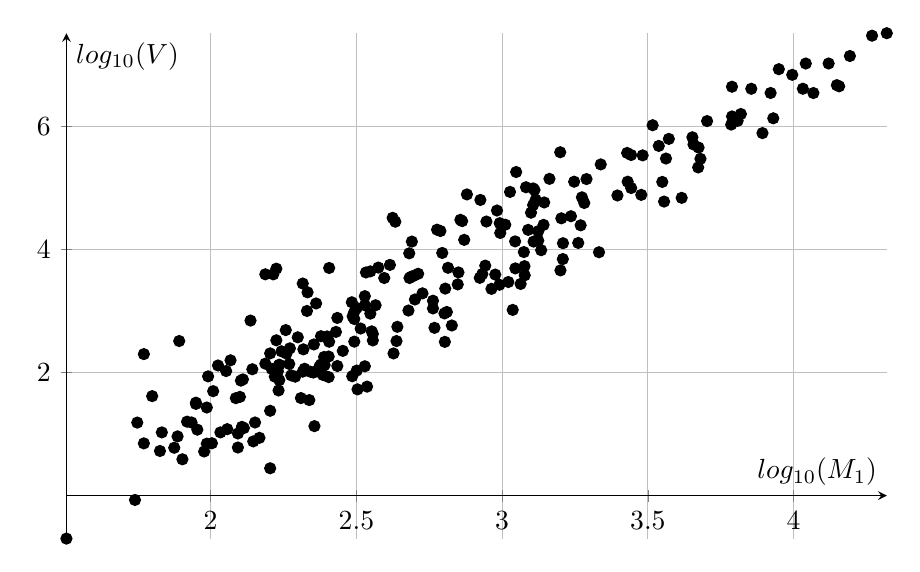
\begin{tikzpicture}
\begin{axis}[width=12cm,height=8cm,
axis lines=middle, xlabel={$log_{10}(M_1)$}, ylabel={$log_{10}(V)$},
xmin=1.5051499783199058, xmax=4.319480828050337,
ymin=-0.6989700043360187, ymax=7.518906770153717,
extra tick style={major grid style=black},grid=major]
\addplot [mark=*, only marks] coordinates {
(2.110589710299249,1.8893017025063101)
(2.02530586526477,2.1161648123118737)
(2.2253092817258624,3.690196080028514)
(1.919078092376074,1.2024201977780304)
(2.3783979009481375,2.132259689531044)
(1.9493900066449126,1.5114377022035417)
(2.5563025007672873,2.6290590146121775)
(3.8930401119571174,5.894521592313384)
(2.827369273053825,2.766366366191725)
(2.2041199826559246,2.313041477993241)
(2.810232517995084,2.986221321921366)
(2.945960703577568,4.456556889858923)
(2.53655844257153,1.7723217067229198)
(2.9319661147281724,3.603570810833047)
(2.3304137733491905,3.0024017071695166)
(3.048053173115609,5.261700987694412)
(2.681241237375587,3.9397355140239028)
(2.624282095835668,4.516641125276831)
(2.762678563727436,3.043885997687633)
(2.187520720836463,3.598681098907163)
(3.9301336458411176,6.135328024033434)
(3.8189513116401725,6.205079897573985)
(1.9867717342662448,1.4326486600131065)
(2.3096301674258983,1.5861651813773168)
(2.187520720836463,2.1455071714096623)
(2.0530784434834195,2.0255984179691437)
(2.3617278360175926,3.1246296093882875)
(3.949194774237982,6.933645525949034)
(2.9934362304976116,4.270899536716091)
(2.850033257689769,3.62935862258034)
(2.2095150145426303,2.060225524394167)
(3.9951962915971793,6.842255669870494)
(2.4533183400470375,2.353723937588949)
(3.077367905284156,3.5823056337991357)
(2.4065401804339546,3.7015679850559273)
(2.086359830674748,1.5846542400042958)
(2.2329961103921536,2.110910222862586)
(3.208710019906401,4.104214833202107)
(1.7993405494535815,1.6174663223227894)
(3.1338581252033344,3.991060867336677)
(3.4426365257822313,5.0012477132165465)
(3.2692793897718984,4.3953798183655985)
(4.2689989585426735,7.4785919782652845)
(2.5289167002776547,3.2433253064048313)
(3.332236415491443,3.957451640973415)
(2.2304489213782737,2.021348352175276)
(3.2030328870147105,4.508943616417986)
(3.010723865391773,4.404937193444941)
(2.633468455579586,4.453807410461225)
(2.4857214264815797,1.9413544870741446)
(1.9542425094393248,1.0725506672154261)
(3.2736955879300917,4.850314498869368)
(3.0362295440862943,3.0197451611626906)
(2.5327543789924976,3.6285539698935225)
(2.8627275283179743,4.46364463341919)
(2.3541084391474008,2.4576490310602934)
(2.804820678721162,3.3661253696265216)
(2.2430380486862944,2.3463529744506384)
(2.7767011839884104,4.324195541965875)
(2.4345689040341987,2.10744390151416)
(3.5162708827293403,6.02280213455429)
(2.3384564936046046,1.5531981666918748)
(2.404833716619938,1.9276674643013594)
(2.487138375477186,2.9149510611278813)
(2.869818207979328,4.158550947069742)
(3.261024833992397,4.108868594335923)
(3.021189299069938,3.473347917960341)
(3.2469906992415494,5.1043407000326795)
(2.3521825181113623,2.0012553521371235)
(4.120014252078067,7.026345332117251)
(1.7708520116421442,2.301029995663981)
(2.3180633349627615,2.3781070625097422)
(2.3729120029701067,2.094988884153331)
(1.8750612633916997,0.7781512503836435)
(2.5289167002776547,3.0950995796456136)
(2.700703717145019,3.1888972496655783)
(3.442322955745574,5.538261383647847)
(2.81424759573192,3.7043333313349556)
(3.703033304733686,6.0899937855546495)
(3.1442627737619904,4.766828386772239)
(2.925312091499649,4.807671991878399)
(3.7884512070234555,6.648699032636881)
(3.854731017213942,6.61545105201613)
(3.162265614298021,5.150568494793861)
(3.1149444157125843,4.8112124638026295)
(2.726727209026572,3.288966121430523)
(4.031650793551264,6.615811349712656)
(1.7708520116421442,0.8495071588315756)
(2.3159703454569174,2.0160241898425677)
(3.0633333589517493,3.4416390361140126)
(2.2355284469075487,2.1285204277315373)
(2.8020892578817325,2.962759882966592)
(2.404833716619938,2.26150077319828)
(1.5051499783199058,-0.6989700043360187)
(2.6148972160331345,3.7516126536562173)
(2.7118072290411908,3.6070754167873944)
(2.963315511386111,3.361809651907951)
(2.093421685162235,0.7820462939763456)
(3.3382572302462554,5.385552504732252)
(3.5493711523331766,5.1009217642820515)
(2.3856062735983117,1.9619979741284004)
(2.923244018630276,3.5410172928456563)
(3.123851640967086,4.299841039569371)
(1.9867717342662448,0.8450980400142567)
(2.008600171761917,1.6983905586147934)
(2.847572659142112,3.434283999039787)
(2.2041199826559246,0.4447181689885548)
(3.20002926655377,3.662411516877962)
(2.1003705451175625,1.6055205234374688)
(2.8567288903828825,4.484465931154977)
(2.803457115648414,2.4999209514943916)
(3.4820155764507117,5.53258298931776)
(2.9916690073799486,4.4295863158722355)
(2.678518379040114,3.0093528203388042)
(3.106190897263415,4.995030190801473)
(3.6737579365495763,5.6591937624128725)
(2.2329961103921536,1.7101173651118162)
(3.6526330680831096,5.826252697358896)
(3.098989639401177,4.6003901802505185)
(2.2988530764097064,2.5740922170633866)
(3.4772659954248524,4.890209444341324)
(3.785756799962643,6.033105739540872)
(2.976349979003273,3.5942733022270197)
(1.8920946026904801,2.513550520346337)
(1.9777236052888476,0.7174534096681198)
(2.2253092817258624,2.5255306856799953)
(2.0681858617461617,2.200224938768488)
(3.106190897263415,4.724916108623423)
(4.319480828050337,7.518906770153717)
(3.788663213120857,6.165561437169954)
(2.4913616938342726,2.9721756022004318)
(3.1078880251827985,4.130724228165944)
(4.04166896647561,7.025922150535285)
(1.7481880270062005,1.187520720836463)
(2.214843848047698,3.5977682933213706)
(3.026941627959029,4.938002817389457)
(3.6565772913961134,5.710334473753581)
(2.2576785748691846,2.691544559996647)
(1.7403626894942439,-0.07058107428570727)
(2.4297522800024076,2.6621416653736167)
(2.5477747053878224,2.9588197569614003)
(2.6821450763738315,3.5387155892481412)
(2.501059262217751,2.0328319929325596)
(2.6901960800285134,4.130709994038458)
(2.5658478186735176,3.0954770343927818)
(2.695481676490197,3.5716942774601916)
(2.2695129442179165,2.140972339302524)
(3.5373152731120094,5.686215711535072)
(3.428782511496954,5.57203525029253)
(4.192957529884656,7.148177996370741)
(2.5477747053878224,3.6462185097533273)
(2.575187844927661,3.7078425891424036)
(2.093421685162235,1.0104027602969754)
(3.3955011243056257,4.880803796054198)
(2.4065401804339546,2.5019923596491322)
(2.7944880466591693,3.945860088342011)
(3.920957705955449,6.546939748123799)
(2.5563025007672873,2.5234342867464368)
(2.6374897295125104,2.5131815933913293)
(3.236033147117636,4.542896746285134)
(2.5526682161121927,2.6705440298657708)
(2.3654879848908994,2.020692678682028)
(3.1992064791616572,5.58324163433773)
(2.143014800254095,2.054883306283622)
(3.11092624226642,4.969853048925632)
(2.2355284469075487,1.877946951629188)
(2.7678976160180904,2.728353782021228)
(3.680335513414563,5.476289871258936)
(2.7881683711411673,4.3025985161739335)
(2.3560258571931225,1.1298988216695378)
(2.8790958795000723,4.897401639443342)
(2.390935107103379,2.1242433089466486)
(1.9912260756924949,1.9390197764486663)
(1.9493900066449126,1.4913616938342726)
(2.501059262217751,3.0505437913005267)
(2.9907826918031377,3.4286507867872538)
(2.1367205671564067,2.8459932798852767)
(2.271841606536499,2.394951732105887)
(2.342422680822206,2.0141438111386196)
(2.1673173347481756,0.9395192526186184)
(2.2600713879850747,2.3105547887740983)
(2.220108088040055,1.9349791314294458)
(1.8325089127062362,1.0280287237359604)
(3.2893659515200313,5.146962281374943)
(3.123851640967086,4.146913191718257)
(2.0043213737826426,0.8512583487190752)
(2.6404814369704215,2.744727494900168)
(2.503790683057181,1.7278331076343305)
(3.0445397603924107,4.133830565731892)
(1.8260748027008262,0.7257631810724322)
(2.9420080530223127,3.739466856356103)
(3.571825249040829,5.800150006002939)
(2.6884198220027105,3.5599963460325896)
(2.5954962218255737,3.5386545102378473)
(2.1461280356782377,0.881691842553922)
(3.0891983668051486,4.321050058646378)
(3.045322978786657,3.69469731223624)
(1.9030899869919433,0.5906804451232659)
(2.3996737214810375,2.588247341812548)
(2.6273658565927325,2.3120715213029315)
(3.074450718954591,3.960485047655226)
(2.107209969647868,1.1179739564353584)
(2.3783979009481375,2.59193522773433)
(4.06774020292624,6.5461988792249155)
(2.1139433523068365,1.0988359341978273)
(2.3891660843645326,2.254427221540668)
(1.9344984512435675,1.189056236092315)
(2.4345689040341987,2.8893311951884435)
(2.514547752660286,2.717080782383067)
(2.276461804173244,1.9551754732533502)
(1.8864907251724818,0.9631973520922511)
(2.484299839346786,3.1436587344094393)
(2.322219294733919,2.062525008876046)
(2.0569048513364723,1.0804274291099996)
(2.2041199826559246,1.3795644887491045)
(2.5289167002776547,2.103251815334661)
(3.2081725266671213,3.846428754772363)
(2.332438459915605,3.305474207654434)
(2.0334237554869494,1.0280287237359604)
(4.148263229636878,6.6743104750179905)
(3.1420764610732843,4.402329459586968)
(3.672467313068082,5.336247054846863)
(3.555457217204649,4.781308249662078)
(4.156094630639427,6.655799142923314)
(3.807805532270624,6.093707734963201)
(3.6158448828747014,4.8417115785119)
(3.430558769522757,5.104286217017372)
(3.0766404436703416,3.7308460003706565)
(2.492760389026837,2.871602121022312)
(3.562054829656378,5.48085802900349)
(2.290034611362518,1.9343498983389538)
(3.081707270097349,5.014215921798604)
(2.1522883443830563,1.1889738194896236)
(2.762678563727436,3.1688179992656647)
(3.2817149700272954,4.758705288570067)
(2.982271233039568,4.635883859129601)
(2.3159703454569174,3.448517380461247)
(2.492760389026837,2.5037437348381983)
(2.103803720955957,1.8698490538656023)
};
\end{axis}\end{tikzpicture}

  \caption{The relationship between the number of files in the repository and its volatility}
  \label{fig:1}
\end{figure}

The Figure~\ref{fig:2} demonstrates the relationship between
the logarithm of the size of the Git repository in bytes~($M_2$) and
the logarithm of its volatility~($V$).
It is visually obvious that
binary-size larger repositories tend to have higher values
of the volatility metric.

\begin{figure}[h]
  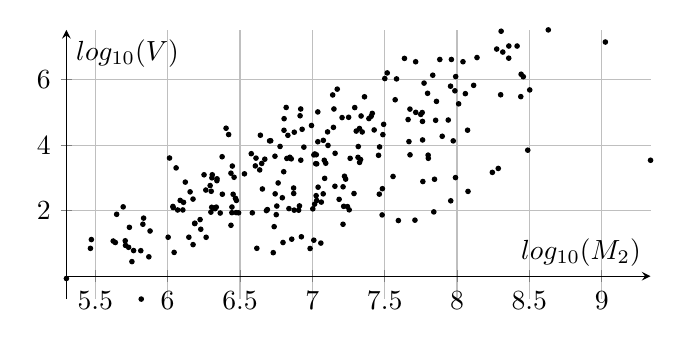
\begin{tikzpicture}
\begin{axis}[width=9cm,height=5cm,
axis lines=middle, xlabel={$log_{10}(M_2)$}, ylabel={$log_{10}(V)$},
xmin=5.300262788643882, xmax=9.337817607630692,
ymin=-0.6989700043360187, ymax=7.518906770153717,
extra tick style={major grid style=black},grid=major]
\addplot [mark=*, only marks, mark size=0.8pt] coordinates {
(5.647511087650302,1.8893017025063101)
(5.692582562274909,2.1161648123118737)
(7.457776654581765,3.690196080028514)
(6.924266515548286,1.2024201977780304)
(7.216770668394846,2.132259689531044)
(6.736250491039094,1.5114377022035417)
(6.263900824669455,2.6290590146121775)
(7.772166756265352,5.894521592313384)
(6.293769252845786,2.766366366191725)
(6.08679853123444,2.313041477993241)
(7.085378962615548,2.986221321921366)
(8.073052438629489,4.456556889858923)
(5.833765270373452,1.7723217067229198)
(6.6106728298275454,3.603570810833047)
(6.30597012059405,3.0024017071695166)
(8.01135938525084,5.261700987694412)
(6.941504326842757,3.9397355140239028)
(6.403689023195856,4.516641125276831)
(7.55794281772462,3.043885997687633)
(7.801742259114062,3.598681098907163)
(7.832429033496079,6.135328024033434)
(7.51781901311406,6.205079897573985)
(6.228963139350912,1.4326486600131065)
(5.8287062875333175,1.5861651813773168)
(6.911021863841136,2.1455071714096623)
(7.254826158872854,2.0255984179691437)
(6.530798713780083,3.1246296093882875)
(8.274468088036434,6.933645525949034)
(7.897747736931188,4.270899536716091)
(6.844839806207417,3.62935862258034)
(6.3274051204258495,2.060225524394167)
(8.316481146610343,6.842255669870494)
(6.175373791317805,2.353723937588949)
(6.854293468338267,3.5823056337991357)
(7.010764072843986,3.7015679850559273)
(7.21217076517489,1.5846542400042958)
(6.444402394827787,2.110910222862586)
(7.03795995395443,4.104214833202107)
(6.187963813507848,1.6174663223227894)
(7.1083857895436475,3.991060867336677)
(7.714825821265492,5.0012477132165465)
(6.8752895843553175,4.3953798183655985)
(8.304971800095547,7.4785919782652845)
(6.636303507733764,3.2433253064048313)
(7.317572660067466,3.957451640973415)
(6.104904475285803,2.021348352175276)
(7.325796058101266,4.508943616417986)
(7.105349074215121,4.404937193444941)
(6.804120410229532,4.453807410461225)
(6.473222079150062,1.9413544870741446)
(5.62369782965714,1.0725506672154261)
(7.250997352029089,4.850314498869368)
(6.459224316888177,3.0197451611626906)
(7.315625731419164,3.6285539698935225)
(7.427477475053893,4.46364463341919)
(7.026496206959709,2.4576490310602934)
(6.6060832766200726,3.3661253696265216)
(7.18526888548742,2.3463529744506384)
(6.421684856027839,4.324195541965875)
(6.335904402636946,2.10744390151416)
(7.582014644162053,6.02280213455429)
(6.437615498426593,1.5531981666918748)
(6.363392521136581,1.9276674643013594)
(6.34035129678636,2.9149510611278813)
(7.762010151213755,4.158550947069742)
(7.667803422511902,4.108868594335923)
(7.326540074714177,3.473347917960341)
(6.919738084515799,5.1043407000326795)
(6.682555250271293,2.0012553521371235)
(8.358266231992452,7.026345332117251)
(7.956847502898422,2.301029995663981)
(6.468604728705185,2.3781070625097422)
(6.038266781443436,2.094988884153331)
(5.8142435991385435,0.7781512503836435)
(6.251518012511634,3.0950995796456136)
(6.802167821086165,3.1888972496655783)
(8.30184972110206,5.538261383647847)
(7.675242757355436,3.7043333313349556)
(8.458299732102924,6.0899937855546495)
(7.939454517948911,4.766828386772239)
(6.804986468601834,4.807671991878399)
(7.636810809124664,6.648699032636881)
(7.881086683344374,6.61545105201613)
(6.819254177642263,5.150568494793861)
(7.390924196641542,4.8112124638026295)
(8.285197877262975,3.288966121430523)
(7.961175323027738,6.615811349712656)
(5.466296585118939,0.8495071588315756)
(6.874497530873762,2.0160241898425677)
(6.6502204611943885,3.4416390361140126)
(6.0362942639242805,2.1285204277315373)
(7.230424676850775,2.962759882966592)
(7.062131249788388,2.26150077319828)
(5.817423886822182,-0.6989700043360187)
(7.1574214368258895,3.7516126536562173)
(6.012874749500376,3.6070754167873944)
(6.447034394923102,3.361809651907951)
(5.764718474842184,0.7820462939763456)
(7.572658071914742,5.385552504732252)
(7.6746820790126336,5.1009217642820515)
(7.839560278999556,1.9619979741284004)
(6.920281564391052,3.5410172928456563)
(6.830978076089829,4.299841039569371)
(6.984383724905092,0.8450980400142567)
(7.594686168986868,1.6983905586147934)
(7.023330954869164,3.434283999039787)
(5.75304426092567,0.4447181689885548)
(6.741791612866611,3.662411516877962)
(6.186993042810472,1.6055205234374688)
(6.9294377787949335,4.484465931154977)
(6.452524568899601,2.4999209514943916)
(7.140766405956862,5.53258298931776)
(7.303517014215802,4.4295863158722355)
(7.989583204791942,3.0093528203388042)
(7.759497575432197,4.995030190801473)
(7.985455216510193,5.6591937624128725)
(7.709384558883058,1.7101173651118162)
(8.115131995079782,5.826252697358896)
(6.994177997738788,4.6003901802505185)
(6.155107289299944,2.5740922170633866)
(7.336993487863417,4.890209444341324)
(7.500784432642139,6.033105739540872)
(6.8240192331184675,3.5942733022270197)
(7.075231819351746,2.513550520346337)
(6.7299284276041655,0.7174534096681198)
(6.8713167196346445,2.5255306856799953)
(7.015821806784398,2.200224938768488)
(7.761494221676318,4.724916108623423)
(8.631002097352543,7.518906770153717)
(8.443188590745871,6.165561437169954)
(6.341315200865003,2.9721756022004318)
(7.974003266097732,4.130724228165944)
(8.415343576497788,7.025922150535285)
(6.265868299473298,1.187520720836463)
(7.261369228169512,3.5977682933213706)
(7.74937309508104,4.938002817389457)
(7.172214636170962,5.710334473753581)
(6.87078272340907,2.691544559996647)
(5.300262788643882,-0.07058107428570727)
(6.654870280891531,2.6621416653736167)
(7.844649063937476,2.9588197569614003)
(9.337817607630692,3.5387155892481412)
(6.689416309290988,2.0328319929325596)
(6.704494726141922,4.130709994038458)
(6.308426740665571,3.0954770343927818)
(6.671462029133507,3.5716942774601916)
(6.7545023758861475,2.140972339302524)
(8.50266545629637,5.686215711535072)
(8.057743581675043,5.57203525029253)
(9.025496341512497,7.148177996370741)
(6.376466544635199,3.6462185097533273)
(7.027448729784829,3.7078425891424036)
(7.058905799011861,1.0104027602969754)
(7.406486341612334,4.880803796054198)
(6.377999766664029,2.5019923596491322)
(7.464750328982202,3.945860088342011)
(8.041238076442523,6.546939748123799)
(7.288091983401679,2.5234342867464368)
(6.743096831936902,2.5131815933913293)
(7.145936779915382,4.542896746285134)
(7.484405922395583,2.6705440298657708)
(6.069144704654302,2.020692678682028)
(7.7966660873049625,5.58324163433773)
(7.003307209436519,2.054883306283622)
(7.414326084467295,4.969853048925632)
(6.750677451375395,1.877946951629188)
(7.212506840030667,2.728353782021228)
(7.360615335985346,5.476289871258936)
(6.6408407489646795,4.3025985161739335)
(6.857624401030012,1.1298988216695378)
(6.915411549923649,4.897401639443342)
(7.242796389648249,2.1242433089466486)
(6.443939333914424,1.9390197764486663)
(5.735553392193666,1.4913616938342726)
(7.222398565686014,3.0505437913005267)
(7.030321652115488,3.4286507867872538)
(6.763654217033682,2.8459932798852767)
(6.792597860384574,2.394951732105887)
(6.905389935573879,2.0141438111386196)
(5.708780255462843,0.9395192526186184)
(7.030208924004791,2.3105547887740983)
(6.4903262792861804,1.9349791314294458)
(5.638301521297118,1.0280287237359604)
(7.293176884526661,5.146962281374943)
(7.076061350348882,4.146913191718257)
(6.616459549203057,0.8512583487190752)
(7.15623928042319,2.744727494900168)
(6.224148579398108,1.7278331076343305)
(6.712339019473114,4.133830565731892)
(6.044794853066763,0.7257631810724322)
(6.577999902780046,3.739466856356103)
(7.955393835994941,5.800150006002939)
(7.333627141970388,3.5599963460325896)
(7.082577289830291,3.5386545102378473)
(5.7300527265942955,0.881691842553922)
(7.487708666654527,4.321050058646378)
(7.800370301408723,3.69469731223624)
(5.870121697786239,0.5906804451232659)
(8.076066245842918,2.588247341812548)
(6.47502245779757,2.3120715213029315)
(6.776950214594808,3.960485047655226)
(5.472753524765399,1.1179739564353584)
(6.301135082213642,2.59193522773433)
(7.714217071699241,6.5461988792249155)
(7.010344104840682,1.0988359341978273)
(6.1096453563010105,2.254427221540668)
(6.146625018391679,1.189056236092315)
(7.764005886984079,2.8893311951884435)
(7.039758047307564,2.717080782383067)
(6.298960218263159,1.9551754732533502)
(6.175587474902988,0.9631973520922511)
(6.437442326282366,3.1436587344094393)
(6.838347348242559,2.062525008876046)
(5.706793713240614,1.0804274291099996)
(5.878410909871675,1.3795644887491045)
(6.304505822597521,2.103251815334661)
(8.48907599373849,3.846428754772363)
(6.058438172384501,3.305474207654434)
(6.797287142515685,1.0280287237359604)
(8.138183053298057,6.6743104750179905)
(7.344702241442134,4.402329459586968)
(7.8580787087941655,5.336247054846863)
(7.662081722840741,4.781308249662078)
(8.357610751942017,6.655799142923314)
(7.991000786832456,6.093707734963201)
(7.205530612054983,4.8417115785119)
(7.149378848203527,5.104286217017372)
(7.016882813474166,3.7308460003706565)
(6.1219794922001,2.871602121022312)
(8.440771127599923,5.48085802900349)
(6.585223889845297,1.9343498983389538)
(7.037747876448219,5.014215921798604)
(6.003347204379362,1.1889738194896236)
(8.244260181749404,3.1688179992656647)
(7.852282308064531,4.758705288570067)
(7.493122782909744,4.635883859129601)
(7.092757547623055,3.448517380461247)
(7.462936697988623,2.5037437348381983)
(7.482397355847451,1.8698490538656023)
};
\end{axis}\end{tikzpicture}

  \caption{The relationship between the size of the Git repository in bytes and its volatility}
  \label{fig:2}
\end{figure}

The Figure~\ref{fig:3} demonstrates the relationship between
the logarithm of the size of the Git repository in bytes~($M_3$) and
the logarithm of its volatility~($V$).
It is visually obvious that
repositories with more directories tend to have higher values
of the volatility metric.

\begin{figure}[h]
  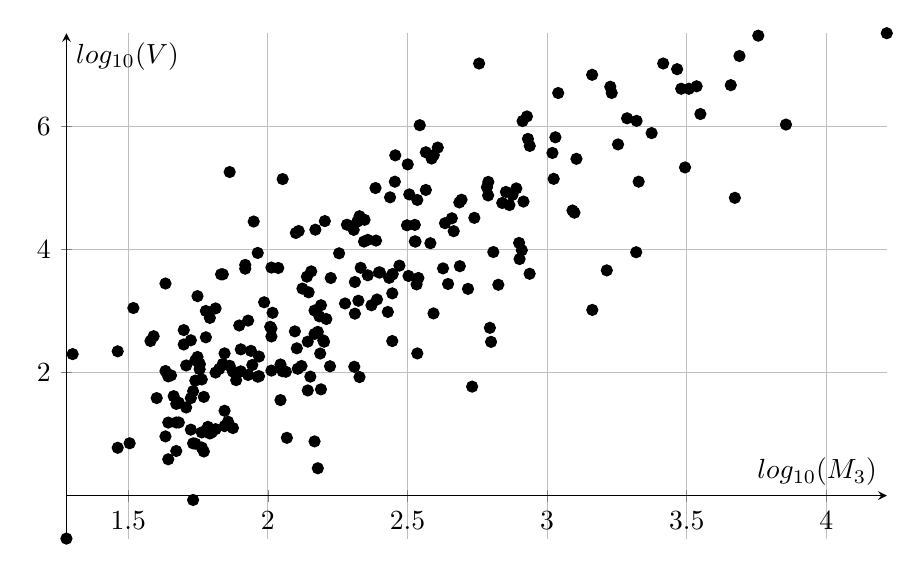
\begin{tikzpicture}
\begin{axis}[width=12cm,height=8cm,
axis lines=middle, xlabel={$log_{10}(M_3)$}, ylabel={$log_{10}(V)$},
xmin=1.2787536009528289, xmax=4.216456214915741,
ymin=-0.6989700043360187, ymax=7.518906770153717,
extra tick style={major grid style=black},grid=major]
\addplot [mark=*, only marks] coordinates {
(1.7634279935629371,1.8893017025063101)
(1.7075701760979363,2.1161648123118737)
(1.919078092376074,3.690196080028514)
(1.8573324964312683,1.2024201977780304)
(2.045322978786657,2.132259689531044)
(1.6812412373755872,1.5114377022035417)
(2.1673173347481756,2.6290590146121775)
(3.374381698050882,5.894521592313384)
(1.8976270912904412,2.766366366191725)
(1.845098040014257,2.313041477993241)
(2.4297522800024076,2.986221321921366)
(1.9493900066449126,4.456556889858923)
(2.7315887651867388,1.7723217067229198)
(2.447158031342219,3.603570810833047)
(1.7781512503836434,3.0024017071695166)
(1.8633228601204557,5.261700987694412)
(2.255272505103306,3.9397355140239028)
(2.7395723444500915,4.516641125276831)
(1.8129133566428552,3.043885997687633)
(1.8388490907372552,3.598681098907163)
(3.2864564697469825,6.135328024033434)
(3.5490032620257876,6.205079897573985)
(1.7075701760979363,1.4326486600131065)
(1.6020599913279623,1.5861651813773168)
(1.7558748556724912,2.1455071714096623)
(1.6334684555795864,2.0255984179691437)
(2.276461804173244,3.1246296093882875)
(3.465680211598278,6.933645525949034)
(2.1003705451175625,4.270899536716091)
(2.397940008672037,3.62935862258034)
(1.8260748027008262,2.060225524394167)
(3.1613680022349744,6.842255669870494)
(1.9395192526186182,2.353723937588949)
(2.3579348470004535,3.5823056337991357)
(2.0374264979406234,3.7015679850559273)
(1.724275869600789,1.5846542400042958)
(1.8633228601204557,2.110910222862586)
(2.5820633629117085,4.104214833202107)
(1.6627578316815739,1.6174663223227894)
(2.909556029241175,3.991060867336677)
(2.3856062735983117,5.0012477132165465)
(2.4983105537896004,4.3953798183655985)
(3.7563317673210572,7.4785919782652845)
(1.7481880270062005,3.2433253064048313)
(3.319106059309776,3.957451640973415)
(2.0530784434834195,2.021348352175276)
(2.658964842664435,4.508943616417986)
(2.2833012287035492,4.404937193444941)
(2.320146286111054,4.453807410461225)
(1.968482948553935,1.9413544870741446)
(1.724275869600789,1.0725506672154261)
(2.437750562820388,4.850314498869368)
(3.1619666163640745,3.0197451611626906)
(2.4014005407815437,3.6285539698935225)
(2.2041199826559246,4.46364463341919)
(1.6989700043360185,2.4576490310602934)
(2.123851640967086,3.3661253696265216)
(1.462397997898956,2.3463529744506384)
(2.170261715394957,4.324195541965875)
(2.1205739312058496,2.10744390151416)
(2.5440680443502752,6.02280213455429)
(2.045322978786657,1.5531981666918748)
(2.3283796034387376,1.9276674643013594)
(2.1846914308175984,2.9149510611278813)
(2.3579348470004535,4.158550947069742)
(2.899820502427096,4.108868594335923)
(2.311753861055754,3.473347917960341)
(2.45484486000851,5.1043407000326795)
(1.8129133566428552,2.0012553521371235)
(3.415807727635543,7.026345332117251)
(1.301029995663981,2.301029995663981)
(1.9030899869919433,2.3781070625097422)
(2.3096301674258983,2.094988884153331)
(1.462397997898956,0.7781512503836435)
(2.371067862271736,3.0950995796456136)
(2.390935107103379,3.1888972496655783)
(2.5943925503754266,5.538261383647847)
(2.332438459915605,3.7043333313349556)
(2.9122220565324155,6.0899937855546495)
(2.6857417386022635,4.766828386772239)
(2.53529412004277,4.807671991878399)
(3.2263420871636304,6.648699032636881)
(3.5078558716958304,6.61545105201613)
(3.0236639181977933,5.150568494793861)
(2.6937269489236466,4.8112124638026295)
(2.4456042032735974,3.288966121430523)
(3.480294460003006,6.615811349712656)
(1.7323937598229684,0.8495071588315756)
(1.8750612633916997,2.0160241898425677)
(2.6454222693490914,3.4416390361140126)
(1.7558748556724912,2.1285204277315373)
(2.5932860670204567,2.962759882966592)
(1.968482948553935,2.26150077319828)
(1.2787536009528289,-0.6989700043360187)
(1.919078092376074,3.7516126536562173)
(2.9375178920173464,3.6070754167873944)
(2.716837723299524,3.361809651907951)
(1.7634279935629371,0.7820462939763456)
(2.501059262217751,5.385552504732252)
(2.789580712164425,5.1009217642820515)
(1.9294189257142926,1.9619979741284004)
(2.4345689040341987,3.5410172928456563)
(2.665580991017953,4.299841039569371)
(1.7403626894942439,0.8450980400142567)
(1.7323937598229684,1.6983905586147934)
(2.5327543789924976,3.434283999039787)
(2.1789769472931693,0.4447181689885548)
(3.213783299335304,3.662411516877962)
(1.7708520116421442,1.6055205234374688)
(2.3463529744506384,4.484465931154977)
(2.7993405494535817,2.4999209514943916)
(2.4563660331290427,5.53258298931776)
(2.634477270160731,4.4295863158722355)
(2.1673173347481756,3.0093528203388042)
(2.889861721258188,4.995030190801473)
(2.608526033577194,5.6591937624128725)
(2.143014800254095,1.7101173651118162)
(3.0297894708318553,5.826252697358896)
(3.09795107099415,4.6003901802505185)
(1.7781512503836434,2.5740922170633866)
(2.876217840591642,4.890209444341324)
(3.8554585803860353,6.033105739540872)
(2.4456042032735974,3.5942733022270197)
(1.57978359661681,2.513550520346337)
(1.7708520116421442,0.7174534096681198)
(1.724275869600789,2.5255306856799953)
(1.7403626894942439,2.200224938768488)
(2.8651039746411278,4.724916108623423)
(4.216456214915741,7.518906770153717)
(2.9278834103307068,6.165561437169954)
(2.0170333392987803,2.9721756022004318)
(2.5289167002776547,4.130724228165944)
(2.7566361082458477,7.025922150535285)
(1.6434526764861872,1.187520720836463)
(1.8325089127062362,3.5977682933213706)
(2.852479993636856,4.938002817389457)
(3.2540644529143377,5.710334473753581)
(1.6989700043360185,2.691544559996647)
(1.7323937598229684,-0.07058107428570727)
(2.1789769472931693,2.6621416653736167)
(2.311753861055754,2.9588197569614003)
(2.5390760987927767,3.5387155892481412)
(2.012837224705172,2.0328319929325596)
(2.34439227368511,4.130709994038458)
(2.1903316981702914,3.0954770343927818)
(2.503790683057181,3.5716942774601916)
(1.8388490907372552,2.140972339302524)
(2.93801909747621,5.686215711535072)
(3.0191162904470725,5.57203525029253)
(3.6888645680547913,7.148177996370741)
(2.1553360374650614,3.6462185097533273)
(2.012837224705172,3.7078425891424036)
(1.7923916894982537,1.0104027602969754)
(2.7888751157754164,4.880803796054198)
(2.2013971243204513,2.5019923596491322)
(1.9637878273455551,3.945860088342011)
(3.231469590430681,6.546939748123799)
(2.1986570869544226,2.5234342867464368)
(2.4456042032735974,2.5131815933913293)
(2.3283796034387376,4.542896746285134)
(2.0969100130080562,2.6705440298657708)
(1.9030899869919433,2.020692678682028)
(2.5658478186735176,5.58324163433773)
(1.7558748556724912,2.054883306283622)
(2.5658478186735176,4.969853048925632)
(1.8864907251724818,1.877946951629188)
(2.7951845896824237,2.728353782021228)
(3.105169427999331,5.476289871258936)
(2.110589710299249,4.3025985161739335)
(1.845098040014257,1.1298988216695378)
(2.506505032404872,4.897401639443342)
(1.9444826721501687,2.1242433089466486)
(1.6434526764861872,1.9390197764486663)
(1.6720978579357173,1.4913616938342726)
(1.5185139398778873,3.0505437913005267)
(2.825426117767823,3.4286507867872538)
(1.9294189257142926,2.8459932798852767)
(2.103803720955957,2.394951732105887)
(2.064457989226918,2.0141438111386196)
(2.0681858617461617,0.9395192526186184)
(2.187520720836463,2.3105547887740983)
(2.1522883443830563,1.9349791314294458)
(1.7634279935629371,1.0280287237359604)
(2.0530784434834195,5.146962281374943)
(2.387389826338729,4.146913191718257)
(1.5051499783199058,0.8512583487190752)
(2.008600171761917,2.744727494900168)
(2.1903316981702914,1.7278331076343305)
(2.5263392773898437,4.133830565731892)
(1.6720978579357173,0.7257631810724322)
(2.4712917110589383,3.739466856356103)
(2.931457870689005,5.800150006002939)
(2.1398790864012365,3.5599963460325896)
(2.2253092817258624,3.5386545102378473)
(2.1673173347481756,0.881691842553922)
(2.3074960379132126,4.321050058646378)
(2.6273658565927325,3.69469731223624)
(1.6434526764861872,0.5906804451232659)
(2.012837224705172,2.588247341812548)
(2.53529412004277,2.3120715213029315)
(2.807535028068853,3.960485047655226)
(1.785329835010767,1.1179739564353584)
(1.591064607026499,2.59193522773433)
(3.0398105541483504,6.5461988792249155)
(1.8750612633916997,1.0988359341978273)
(1.7481880270062005,2.254427221540668)
(1.6812412373755872,1.189056236092315)
(1.7923916894982537,2.8893311951884435)
(2.012837224705172,2.717080782383067)
(1.6532125137753435,1.9551754732533502)
(1.6334684555795864,0.9631973520922511)
(1.9867717342662448,3.1436587344094393)
(2.107209969647868,2.062525008876046)
(1.8129133566428552,1.0804274291099996)
(1.845098040014257,1.3795644887491045)
(2.2227164711475833,2.103251815334661)
(2.9014583213961123,3.846428754772363)
(2.1461280356782377,3.305474207654434)
(1.7993405494535815,1.0280287237359604)
(3.657820456015697,6.6743104750179905)
(2.5263392773898437,4.402329459586968)
(3.4940153747571436,5.336247054846863)
(2.9153998352122694,4.781308249662078)
(3.5355472791766673,6.655799142923314)
(3.3205616801952362,6.093707734963201)
(3.672467313068082,4.8417115785119)
(3.3279716236230104,5.104286217017372)
(2.687528961214634,3.7308460003706565)
(2.2095150145426303,2.871602121022312)
(2.5865873046717547,5.48085802900349)
(1.9637878273455551,1.9343498983389538)
(2.784617292632875,5.014215921798604)
(1.6720978579357173,1.1889738194896236)
(2.3242824552976926,3.1688179992656647)
(2.839478047374198,4.758705288570067)
(3.0909630765957314,4.635883859129601)
(1.6334684555795864,3.448517380461247)
(2.143014800254095,2.5037437348381983)
(1.7403626894942439,1.8698490538656023)
};
\end{axis}\end{tikzpicture}

  \caption{The relationship between the number of repositories in the repository and its volatility}
  \label{fig:3}
\end{figure}

\section{Conclusion}

A new source code volatility metric was introduced and applied
to \thetotalrepos{} open source Java repositories from GitHub. It was
empirically demonstrated that larger repositories have higher values
of the volatility metric.

The source code of Ruby and Python scripts used to do the research
is available in GitHub repository \texttt{yegor256/volatility-vs-size}.

\bibliography{main}

\end{document}
